% ============================================================
\chapter{Asymmetric Topology in Theoretical CS}
\label{ch:theoretical_cs}
% ============================================================

In 1969, Dana Scott, confronted with the problem of giving mathematical meaning to Church's lambda calculus, sought a space $D$ isomorphic to its own space of continuous functions $D \to D$. Classical Hausdorff topological spaces would not do --- such an isomorphism is impossible there for cardinality reasons. Scott discovered that the solution lies in \emph{continuous lattices} equipped with their Scott topology, a resolutely non-Hausdorff topology where open sets represent the ``observable'' properties of a computation. This discovery founded \emph{denotational semantics}, the bridge between program logic and continuous mathematics. This chapter shows how asymmetric topology --- quasi-metrics, $T_0$ spaces, the Scott topology --- constitutes the natural language of theoretical computer science.

\begin{intuition}
Domain theory, born from the work of Dana Scott in the 1960s--70s, provides a mathematical
model for the denotational semantics of programming languages. The central idea is that
elements of a domain represent partial ``levels of information,'' and the order reflects
information refinement. The Scott topology, which is non-Hausdorff, captures exactly the
observability properties in a program. This chapter presents these applications of
non-Hausdorff topology to theoretical computer science.
\end{intuition}

% ------------------------------------------------------------
\section{Scott Domains and Denotational Semantics}
% ------------------------------------------------------------

\begin{definition}[Directed set and dcpo]
\index{dcpo}
\index{directed set}
A subset $D$ of a partially ordered set $(P, \leq)$ is \emph{directed} if it is nonempty
and for all $x, y \in D$, there exists $z \in D$ such that $x \leq z$ and $y \leq z$.
A \emph{dcpo} (directed-complete partial order) is a partially ordered set in which every
directed subset has a supremum.
\end{definition}

\begin{definition}[Scott topology]
\index{Scott topology}
Let $(P, \leq)$ be a dcpo. A subset $U \subseteq P$ is \emph{Scott-open} if:
\begin{enumerate}
  \item $U$ is an upper set: $x \in U$ and $x \leq y$ imply $y \in U$;
  \item $U$ is inaccessible by directed suprema: if $D$ is directed and
    $\bigvee D \in U$, then $D \cap U \neq \emptyset$.
\end{enumerate}
\end{definition}

\begin{proposition}
The Scott-open sets on a dcpo $P$ form a topology. This topology is $T_0$ and its
specialization order coincides with the order $\leq$ of $P$.
\end{proposition}

\begin{proof}
The sets $P$ and $\emptyset$ are Scott-open. The finite intersection of Scott-open sets is
Scott-open: the upper set condition is preserved by intersection, and if
$\bigvee D \in U_1 \cap U_2$, then $D \cap U_1$ is cofinal in $D$ and
$D \cap U_1 \cap U_2$ is nonempty. The arbitrary union of Scott-open sets is clearly
Scott-open.

For the specialization order: $x \leq y$ in the order of $P$ if and only if every open
set containing $x$ contains $y$, which is exactly the definition of the specialization
order.
\end{proof}

% Hasse diagram of the flat Boolean domain
\begin{center}
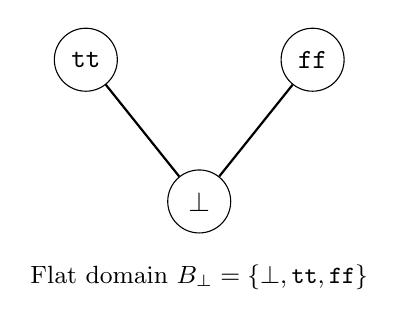
\begin{tikzpicture}[scale=1.2, every node/.style={circle, draw, minimum size=8mm, inner sep=1pt}]
  % Nodes
  \node (bot) at (0,0) {$\bot$};
  \node (tt) at (-1.2,1.5) {$\mathtt{tt}$};
  \node (ff) at (1.2,1.5) {$\mathtt{ff}$};
  % Hasse diagram edges
  \draw[thick] (bot) -- (tt);
  \draw[thick] (bot) -- (ff);
  % Caption
  \node[draw=none, rectangle, minimum size=0pt] at (0,-0.8)
    {\small Flat domain $\mathbb{B}_\bot = \{\bot, \mathtt{tt}, \mathtt{ff}\}$};
\end{tikzpicture}
\end{center}

\begin{definition}[Scott-continuous function]
\index{Scott-continuous function}
Let $(P, \leq_P)$ and $(Q, \leq_Q)$ be dcpos. A function $f\colon P \to Q$ is
\emph{Scott-continuous} if it is monotone and preserves directed suprema: for every
directed subset $D \subseteq P$,
\[
  f\!\left(\bigvee D\right) = \bigvee f(D).
\]
\end{definition}

\begin{proposition}
A function between dcpos is Scott-continuous if and only if it is continuous for the
Scott topologies.
\end{proposition}

\begin{theorem}[Category of dcpos]
The category $\mathbf{DCPO}$ whose objects are dcpos and whose morphisms are
Scott-continuous functions is Cartesian closed. The function space $[P \to Q]$ is the dcpo
of Scott-continuous functions from $P$ to $Q$, ordered pointwise.
\end{theorem}

\begin{proof}[Proof sketch]
The key step is showing that $[P \to Q]$ with the pointwise order
($f \leq g \iff \forall x,\, f(x) \leq g(x)$) is a dcpo. Given a directed family
$(f_i)_{i \in I}$ in $[P \to Q]$, one defines $f = \bigvee f_i$ pointwise by
$f(x) = \bigvee_i f_i(x)$; Scott-continuity of $f$ follows from the interchange of
directed suprema. For Cartesian closedness, one must show that the evaluation map
$\mathrm{ev} \colon [P \to Q] \times P \to Q$ is Scott-continuous: if $U$ is
Scott-open in $Q$, then $\mathrm{ev}^{-1}(U)$ is Scott-open in $[P \to Q] \times P$.
This holds because the preimage of a Scott-open set under evaluation is a union of
rectangles of the form $\{f : f(x) \in U\} \times V$, each of which is Scott-open.
See \textsc{Abramsky--Jung}, \emph{Domain Theory}, Handbook of Logic in Computer
Science, vol.~3, 1994.
\end{proof}

% ------------------------------------------------------------
\section{Domains for the Lambda Calculus}
% ------------------------------------------------------------

\begin{definition}[Continuous domain]
\index{continuous domain}
A dcpo $D$ is a \emph{continuous domain} if for every $x \in D$,
\[
  {\Downarrow} x = \{ a \in D : a \ll x \}
\]
is directed and $x = \bigvee {\Downarrow} x$, where $a \ll x$ means that $a$ is
\emph{way below} $x$ (compact relative to $x$).
\end{definition}

\begin{theorem}[Scott's model of the untyped lambda calculus]
\label{thm:scott-model}
There exists a continuous domain $D_\infty$ such that
\[
  D_\infty \cong [D_\infty \to D_\infty]
\]
in the category of continuous domains with Scott-continuous functions. Such a domain
provides a model for the denotational semantics of the untyped lambda calculus.
\end{theorem}

\begin{proof}[Proof sketch]
One constructs $D_\infty$ as a projective limit of a sequence
$D_0 \leftarrow D_1 \leftarrow D_2 \leftarrow \cdots$ where $D_0 = \{\bot\}$ and
$D_{n+1} = [D_n \to D_n]$, with the arrows being retractions (projection/section pairs).
The projective limit in $\mathbf{DCPO}$ is a dcpo whose elements are coherent sequences
$(x_0, x_1, \ldots)$ with $\pi_n(x_{n+1}) = x_n$. The isomorphism
$D_\infty \cong [D_\infty \to D_\infty]$ follows from the continuity of the functor
$[\cdot \to \cdot]$ on projective limits.
\end{proof}

\begin{intuition}
Scott's model solves a fundamental problem: in naive set theory, there is no set $D$ such
that $D \cong D^D$ (by a cardinality argument, unless $D$ is a singleton). By passing to
dcpos and continuous functions, one escapes this constraint because $[D \to D]$ contains
only the continuous functions, not all functions.
\end{intuition}

\begin{definition}[Denotational interpretation]
\index{denotational semantics}
In a Scott model $D_\infty$, each closed term $M$ of the lambda calculus receives an
interpretation $\llbracket M \rrbracket \in D_\infty$:
\begin{itemize}
  \item $\llbracket x \rrbracket_\rho = \rho(x)$ where $\rho$ is an environment;
  \item $\llbracket \lambda x.\, M \rrbracket_\rho = d \mapsto \llbracket M \rrbracket_{\rho[x \mapsto d]}$;
  \item $\llbracket M N \rrbracket_\rho = \llbracket M \rrbracket_\rho (\llbracket N \rrbracket_\rho)$.
\end{itemize}
\end{definition}

% ------------------------------------------------------------
\section{Continuous Lattices and Programming Language Theory}
% ------------------------------------------------------------

\begin{definition}[Continuous lattice]
\index{continuous lattice}
A complete lattice $L$ is \emph{continuous} if it is a continuous domain, i.e., if for
every $x \in L$, $x = \bigvee \{a \in L : a \ll x\}$.
\end{definition}

\begin{theorem}[Lawson's characterization theorem]
A complete lattice $L$ is continuous if and only if the function
$x \mapsto {\Downarrow} x$ is an isomorphism from $L$ onto a sublattice of the lattice
of ideals of the basis of $L$.
\end{theorem}

\begin{proposition}[Continuous lattices and types]
In denotational semantics:
\begin{itemize}
  \item Base types (integers, Booleans) are interpreted by flat algebraic domains (domains
    with a bottom element $\bot$ and incomparable maximal elements).
  \item The function type $A \to B$ is interpreted by $[D_A \to D_B]$.
  \item Recursive types $T = F(T)$ are interpreted by solutions of domain equations,
    obtained as projective limits.
\end{itemize}
\end{proposition}

% ------------------------------------------------------------
\section{Powerdomains}
% ------------------------------------------------------------

\begin{definition}[Powerdomains]
\index{powerdomain}
Let $D$ be a domain. The \emph{powerdomains} extend $D$ to model nondeterminism. There
are three variants, corresponding to three different observations:
\end{definition}

\begin{definition}[Hoare (lower) powerdomain]
\index{powerdomain!Hoare}
The \emph{Hoare powerdomain} $\mathcal{H}(D)$ is the dcpo of nonempty closed sets of $D$
(in the Scott topology), ordered by:
\[
  A \leq_H B \quad \Longleftrightarrow \quad A \subseteq {\downarrow} B.
\]
Intuitively, $A \leq_H B$ means that every possible result of $A$ is approximated by a
result of $B$. This captures ``partial correctness'' (safety).
\end{definition}

\begin{definition}[Smyth (upper) powerdomain]
\index{powerdomain!Smyth}
The \emph{Smyth powerdomain} $\mathcal{S}(D)$ is the set of nonempty saturated compact
sets of $D$, ordered by reverse inclusion:
\[
  Q_1 \leq_S Q_2 \quad \Longleftrightarrow \quad Q_2 \subseteq Q_1.
\]
This captures ``termination'' (liveness): $Q_1 \leq_S Q_2$ means that the set of possible
behaviors shrinks.
\end{definition}

\begin{definition}[Plotkin (convex) powerdomain]
\index{powerdomain!Plotkin}
The \emph{Plotkin powerdomain} $\mathcal{P}\ell(D)$ combines both orderings:
\[
  A \leq_P B \quad \Longleftrightarrow \quad A \leq_H B \text{ and } A \leq_S B.
\]
This is the Egli-Milner order. It captures both partial correctness and termination.
\end{definition}

\begin{theorem}[Properties of powerdomains]
Let $D$ be a continuous domain.
\begin{enumerate}
  \item $\mathcal{H}(D)$ is a dcpo (under mild hypotheses).
  \item $\mathcal{S}(D)$ is a dcpo if $D$ is coherent (the intersection of saturated
    compact sets is a saturated compact set).
  \item If $D$ is a Scott domain (continuous domain with a countable basis), all three
    powerdomains are continuous domains.
\end{enumerate}
\end{theorem}

\begin{example}
Consider the flat Boolean domain $\mathbb{B}_\bot = \{\bot, \mathtt{true},
\mathtt{false}\}$. Then:
\begin{itemize}
  \item $\mathcal{H}(\mathbb{B}_\bot)$ contains the closed sets: $\{\bot\}$,
    $\{\bot, \mathtt{true}\}$, $\{\bot, \mathtt{false}\}$,
    $\{\bot, \mathtt{true}, \mathtt{false}\}$.
  \item $\mathcal{S}(\mathbb{B}_\bot)$ contains the saturated compact sets:
    $\mathbb{B}_\bot$, $\{\mathtt{true}\}$, $\{\mathtt{false}\}$,
    $\{\mathtt{true}, \mathtt{false}\}$.
\end{itemize}
\end{example}

% ------------------------------------------------------------
\section{Topological Models of Computation}
% ------------------------------------------------------------

\begin{definition}[Effectively presented space]
\index{effectively presented space}
A domain $D$ is \emph{effectively presented} if it has a countable basis $(b_n)_{n \in \N}$
such that the relations $b_n \leq b_m$ and $b_n \ll b_m$ are decidable (semi-decidable
for $\ll$).
\end{definition}

\begin{theorem}[Computability--continuity equivalence]
On an effectively presented domain $D$, the computable functions $D \to D$ (in the sense
of Type-2 computability theory) coincide with the effectively given Scott-continuous
functions.
\end{theorem}

\begin{proposition}[Name spaces and domains]
The B\"ohm domain $\mathcal{B}$ of B\"ohm trees of the lambda calculus is a continuous
domain such that:
\begin{itemize}
  \item Finite elements are finite B\"ohm trees (with $\bot$ at the leaves).
  \item The order is information refinement: $t \leq s$ if $s$ is obtained by replacing
    some $\bot$'s in $t$ with subtrees.
  \item The Scott topology captures exactly observation by head contexts.
\end{itemize}
\end{proposition}

\begin{theorem}[Adequacy and full abstraction]
For the pure lambda calculus, the denotational semantics in a continuous Scott domain is:
\begin{enumerate}
  \item \emph{Adequate}: if $\llbracket M \rrbracket \leq \llbracket N \rrbracket$, then
    $M$ is approximated by $N$ in the operational sense.
  \item \emph{Fully abstract} for filter models: the denotational order coincides with the
    operational preorder.
\end{enumerate}
\end{theorem}

\begin{keyformulas}[title=\textbf{Topology--computer science correspondence}]
\begin{center}
\renewcommand{\arraystretch}{1.3}
\begin{tabular}{|l|l|}
\hline
\textbf{Topological concept} & \textbf{Computer science concept} \\
\hline
Scott-open set & Semi-decidable property \\
Scott-closed set & Limit-verifiable property \\
Saturated compact set & Co-semi-decidable property \\
Continuous function & Program (computable function) \\
$T_0$ topology & Observational distinguishability \\
Bottom element $\bot$ & Divergence / nontermination \\
Directed supremum & Limit of finite approximations \\
\hline
\end{tabular}
\end{center}
\end{keyformulas}

% ------------------------------------------------------------
\section{Exercises}
% ------------------------------------------------------------

\begin{exercise}
Show that the Scott topology on $(\N, \leq)$ is the cofinite topology on $\N$.
\end{exercise}

\begin{exercise}
Let $D = \N \cup \{\infty\}$ equipped with the usual order. Determine the Scott topology,
verify that it is sober and locally compact, and compute the saturated compact sets.
\end{exercise}

\begin{exercise}
Show that the space $[D \to D]$ of Scott-continuous functions from a dcpo $D$ to itself,
equipped with the pointwise order, is a dcpo. Deduce that the category $\mathbf{DCPO}$ is
Cartesian closed.
\end{exercise}

\begin{exercise}
Let $D$ be the flat natural numbers domain $\N_\bot$. Describe explicitly the elements of
the Hoare powerdomain $\mathcal{H}(D)$ and the Smyth powerdomain $\mathcal{S}(D)$.
\end{exercise}

\begin{exercise}
Let $f\colon D \to D$ be a Scott-continuous function on a pointed dcpo $D$ (with $\bot$).
Using Kleene's theorem (Chapter~\ref{ch:fixed_points}), show that the semantics of a
\texttt{while} loop can be defined as the least fixed point of a continuous operator.
\end{exercise}

\begin{exercise}[Powerdomain and monad]
Show that the Hoare powerdomain $\mathcal{H}$ defines a functor
$\mathcal{H}\colon \mathbf{DCPO} \to \mathbf{DCPO}$. Verify that the unit
$\eta_D\colon D \to \mathcal{H}(D)$ defined by $\eta_D(d) = {\downarrow} d$ and the
multiplication $\mu_D\colon \mathcal{H}(\mathcal{H}(D)) \to \mathcal{H}(D)$ defined by
$\mu_D(\mathcal{A}) = \bigcup_{A \in \mathcal{A}} A$ make $\mathcal{H}$ into a monad.
\end{exercise}
